\Exercise  
Considerem una població de ratolins que es troba en una illa deserta. La població inicial de ratolins és de 100 individus. La taxa de creixement natural anual és del 30\% ($r = 0.30$). 

Es vol determinar el temps necessari perquè la població arribi a 1 milió de ratolins en dos casos:

\begin{itemize}
    \item \textbf{Sense aportacions externes:} Només es considera el creixement natural de la població.
    \item \textbf{Amb aportacions externes:} Cada any arriben 20 ratolins nous a més del creixement natural.
\end{itemize}


\Answer


\textbf{Sense Aportacions Externes}

La població en temps $t$ es modela amb l'equació de creixement exponencial:
\[
P(t) = P_0 \cdot (1 + r)^t
\]
ja que cada pas implica:
\[
P(t+1) = P(t) \cdot (1 + r)
\]
On:
\begin{itemize}
    \item $P_0 = 100$ (població inicial)
    \item $r = 0.30$ (taxa de creixement)
    \item $P(t) = 1{,}000{,}000$ (població objectiu)
\end{itemize}

Per trobar el temps $t$ necessari per arribar a 1 milió de ratolins, resolem:
\[
1{,}000{,}000 = 100 \cdot (1.30)^t
\]
\[
10{,}000 = (1.30)^t
\]
Aplicant logaritmes:
\[
\ln(10{,}000) = t \cdot \ln(1.30)
\]
\[
t = \frac{\ln(10{,}000)}{\ln(1.30)} \approx \frac{9.21034}{0.26236} \approx 35.11
\]
Per tant, el temps necessari és aproximadament \textbf{35 anys}.

\textbf{Amb Aportacions Externes}

Amb aportacions externes, la població es modela amb l'equació:
\[
P(t+1) = P(t) \cdot (1 + r) + A
\]
o bé
\[
P(t) = P_0 \cdot (1 + r)^t + A \cdot \frac{(1 + r)^t - 1}{r}
\]
On:
\begin{itemize}
    \item $P_0 = 100$ (població inicial)
    \item $r = 0.30$ (taxa de creixement)
    \item $A = 20$ (aportacions externes)
    \item $P(t) = 1{,}000{,}000$ (població objectiu)
\end{itemize}

Utilitzant un enfocament iteratiu, s'ha de trobar el temps $t$ per al qual la població supera 1 milió de ratolins. En aquest cas, el càlcul és:
\[
P(t) = 100 \cdot (1.30)^t + 20 \cdot \frac{(1.30)^t - 1}{0.30}
\]
Després de calcular iterativament, es troba que el temps necessari és aproximadament \textbf{34 anys}.


El següent gràfic mostra l'evolució de la població amb i sense aportacions externes al llarg del temps:

\begin{minipage}[t]{\linewidth}
  \vspace{-2ex}
  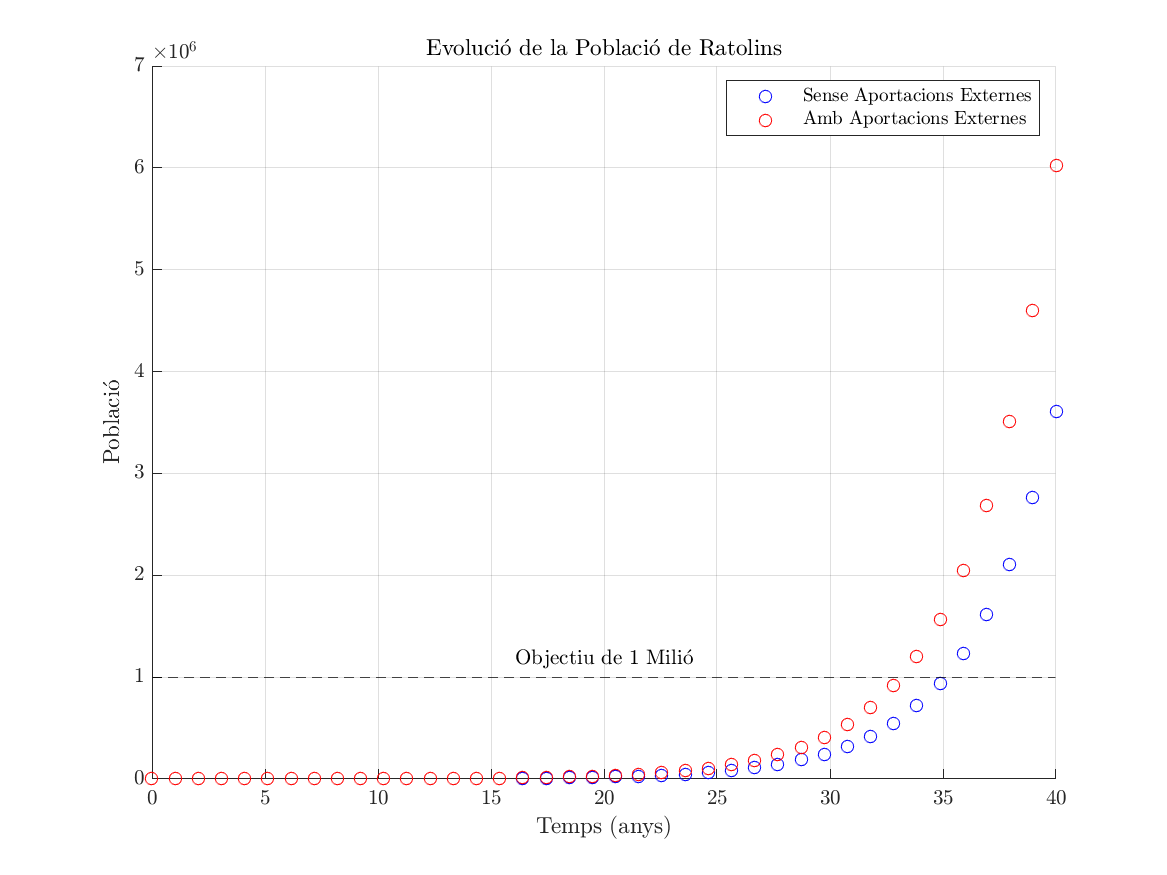
\includegraphics[width=0.8\textwidth]{MalthusRatolins}
  \captionof{figure}{Evolució de la població de ratolins amb i sense aportacions externes. La línia horitzontal indica l'objectiu de 1 milió de ratolins.}
  \label{fig:MalthusRatolins}
\end{minipage}


\blacksquare 